% !TEX TS-program = xelatex
% !TEX encoding = UTF-8 Unicode

\providecommand{\home}{../..}
\documentclass[\home/main.tex]{subfiles}

\begin{document}

\chapter{Background and review of related work} \label{ch:lit}

The goal of the following chapter is to provide the preliminaries and a review of relevant work in the field of robotic manipulation of deformable objects. To provide some historical context, we first discuss how \emph{standard robotic manipulation pipelines} can be used for manipulating deformable objects in \cref{sec:lit_traditional}. Next, in \cref{sec:lit_learning}, we introduce how the inherent limitations of engineered motor control architectures can be overcome by using \emph{learning-based methods}. We break this section down into subsections introducing supervised learning, deep neural networks and reinforcement learning. This is followed by surveying their applications in recent robotic manipulation work. Given the general property that learning-based methods are data-hungry, we continue this discussion by reviewing the role of \emph{large datasets} for robotic learning in \cref{sec:lit_datasets}. An alternative approach to generating data is to use synthetic data. To this end, we discuss the role of \emph{simulation} and the corresponding transferability problems in \cref{sec:lit_simulation}. Critical to robotic learning of manipulation skills is some metric of task success, generally labelled as reward function. The role and methods to obtain \emph{reward functions} for robotic learning, and deformable objects manipulation in particular, is reviewed in \cref{sec:lit_reward_learning}. Finally, we discuss the idea and corresponding literature of \emph{instrumenting the process with sensors} to facilitate the learning process in the manipulation environment in \cref{sec:lit_instrumentation}.

\section{Manipulating deformable objects} \label{sec:lit_traditional}

This section provides important historical context and prior work in the rigid and deformable object manipulation literature. First, we discuss the traditional control approach to rigid object manipulation for robots and how these methods are challenging to generalize towards deformable object manipulation. Next, we provide a definition and categorization of deformable objects. For each category, we provide common tasks and solutions identified in literature.

\subsection{Manipulating rigid objects}
Grasping and manipulation problems in robotics are traditionally solved by manually engineering subsystems for perception, planning and control \autocite{Siciliano2008}. A popular approach is using images as input observation to control the robot's motions. This approach is motivated by the advantage that images enable closed-loop control: non-contact and real-time measurements of the environment can be used to provide feedback to the motion trajectory of the robot. This principle is generally known as visual servoing \autocite{Hutchinson1996} and was first introduced in~\citeyear{Hill1979} by \textcite{Hill1979}. An archetypical pipeline consists of the following steps to grasp and manipulate an object \autocite{Corke1996}. First, observations such as images are used to estimate the state of the object. This state estimation stage usually executes pixel manipulations and image filtering in order to extract features. This object state is used to interpret the scene to calculate the relative position of the target object from the robot end-effector. Once the object is identified, it can be modelled to identify a suitable grasping point. Next, these grasping points are given to a motion planning system that calculates a trajectory to move the end-effector to the desired position and orientation. Finally, a low-level controller sends motor commands to the actuators to move the robot. An example of this archetype control pipeline is displayed in \cref{fig:canonical_robotic_manipulation_engineered_pipeline}.

\begin{figure}[p]
    \centering
    \subfile{figures/canonical-robotic-manipulation-pipeline/fig-canonical-robotic-manipulation-pipeline.tex}
    \vspace*{-10mm}
    \caption[Canonical engineered manipulation pipeline.]{\textbf{Canonical engineered manipulation pipeline with examples of each module.} Cameras record observations that are used to estimate the state of the cloth downstream. The modelling module calculates the deformations on the cloth if certain manipulations are executed. A planning module calculates the desired end-effector trajectory and sends the corresponding joint position to a low-level controller.
    }
    \label{fig:canonical_robotic_manipulation_engineered_pipeline}
\end{figure}

% Probleem met traditionele pipelines toepassen voor vervormbare objecten
Engineering modular, hand-tuned motor control pipelines have been successful for applications in manufacturing \autocite{Clocksin1985,Mochizuki1987}, car steering \autocite{Dickmanns1988}, robotic ping-pong \autocite{Andersson1987}, juggling \autocite{Rizzi1993} as well as fruit picking \autocite{Harrell1989}. However, all of these applications operate under the condition of rigid objects: the shape of the object will not change on contact.
When manipulating objects, this is of importance for determining stable grasping points. More concretely, restraining rigid objects relies on \textit{form closure} \autocite{Nguyen1988} or \textit{force closure} \autocite{Bicchi1995}: fully constraining relative motion of the object or having contact points that can counteract an external wrench through friction.
However, in the case of deformable objects, the object can deform during grasping and manipulation. This leads to exponentially higher dimensional configuration spaces compared to rigid object manipulation \autocite{Foresti2004}. For example, achieving form closure becomes impossible as it requires immobilizing every degree of freedom. Similarly, force closure becomes computationally intractable as it requires constantly incorporating the adapted shape of the object. For example, we visually show (\cref{fig:force_closure_deform_object}) the deformations that occur when grasping a plastic cup versus a rigid glass when trying to achieve force closure. Furthermore, manipulation requires reasoning about the target shape of the object. These properties make many rigid object manipulation techniques hard to extend in the deformable object domain. Unfortunately, to date, the vast majority of robotic manipulation work deals with rigid objects whereas many objects are of deformable nature \autocite{Siciliano2008}.

\begin{figure}[htbp]
    \centering

    \begin{subfigure}[b]{0.95\textwidth}
        \centering
        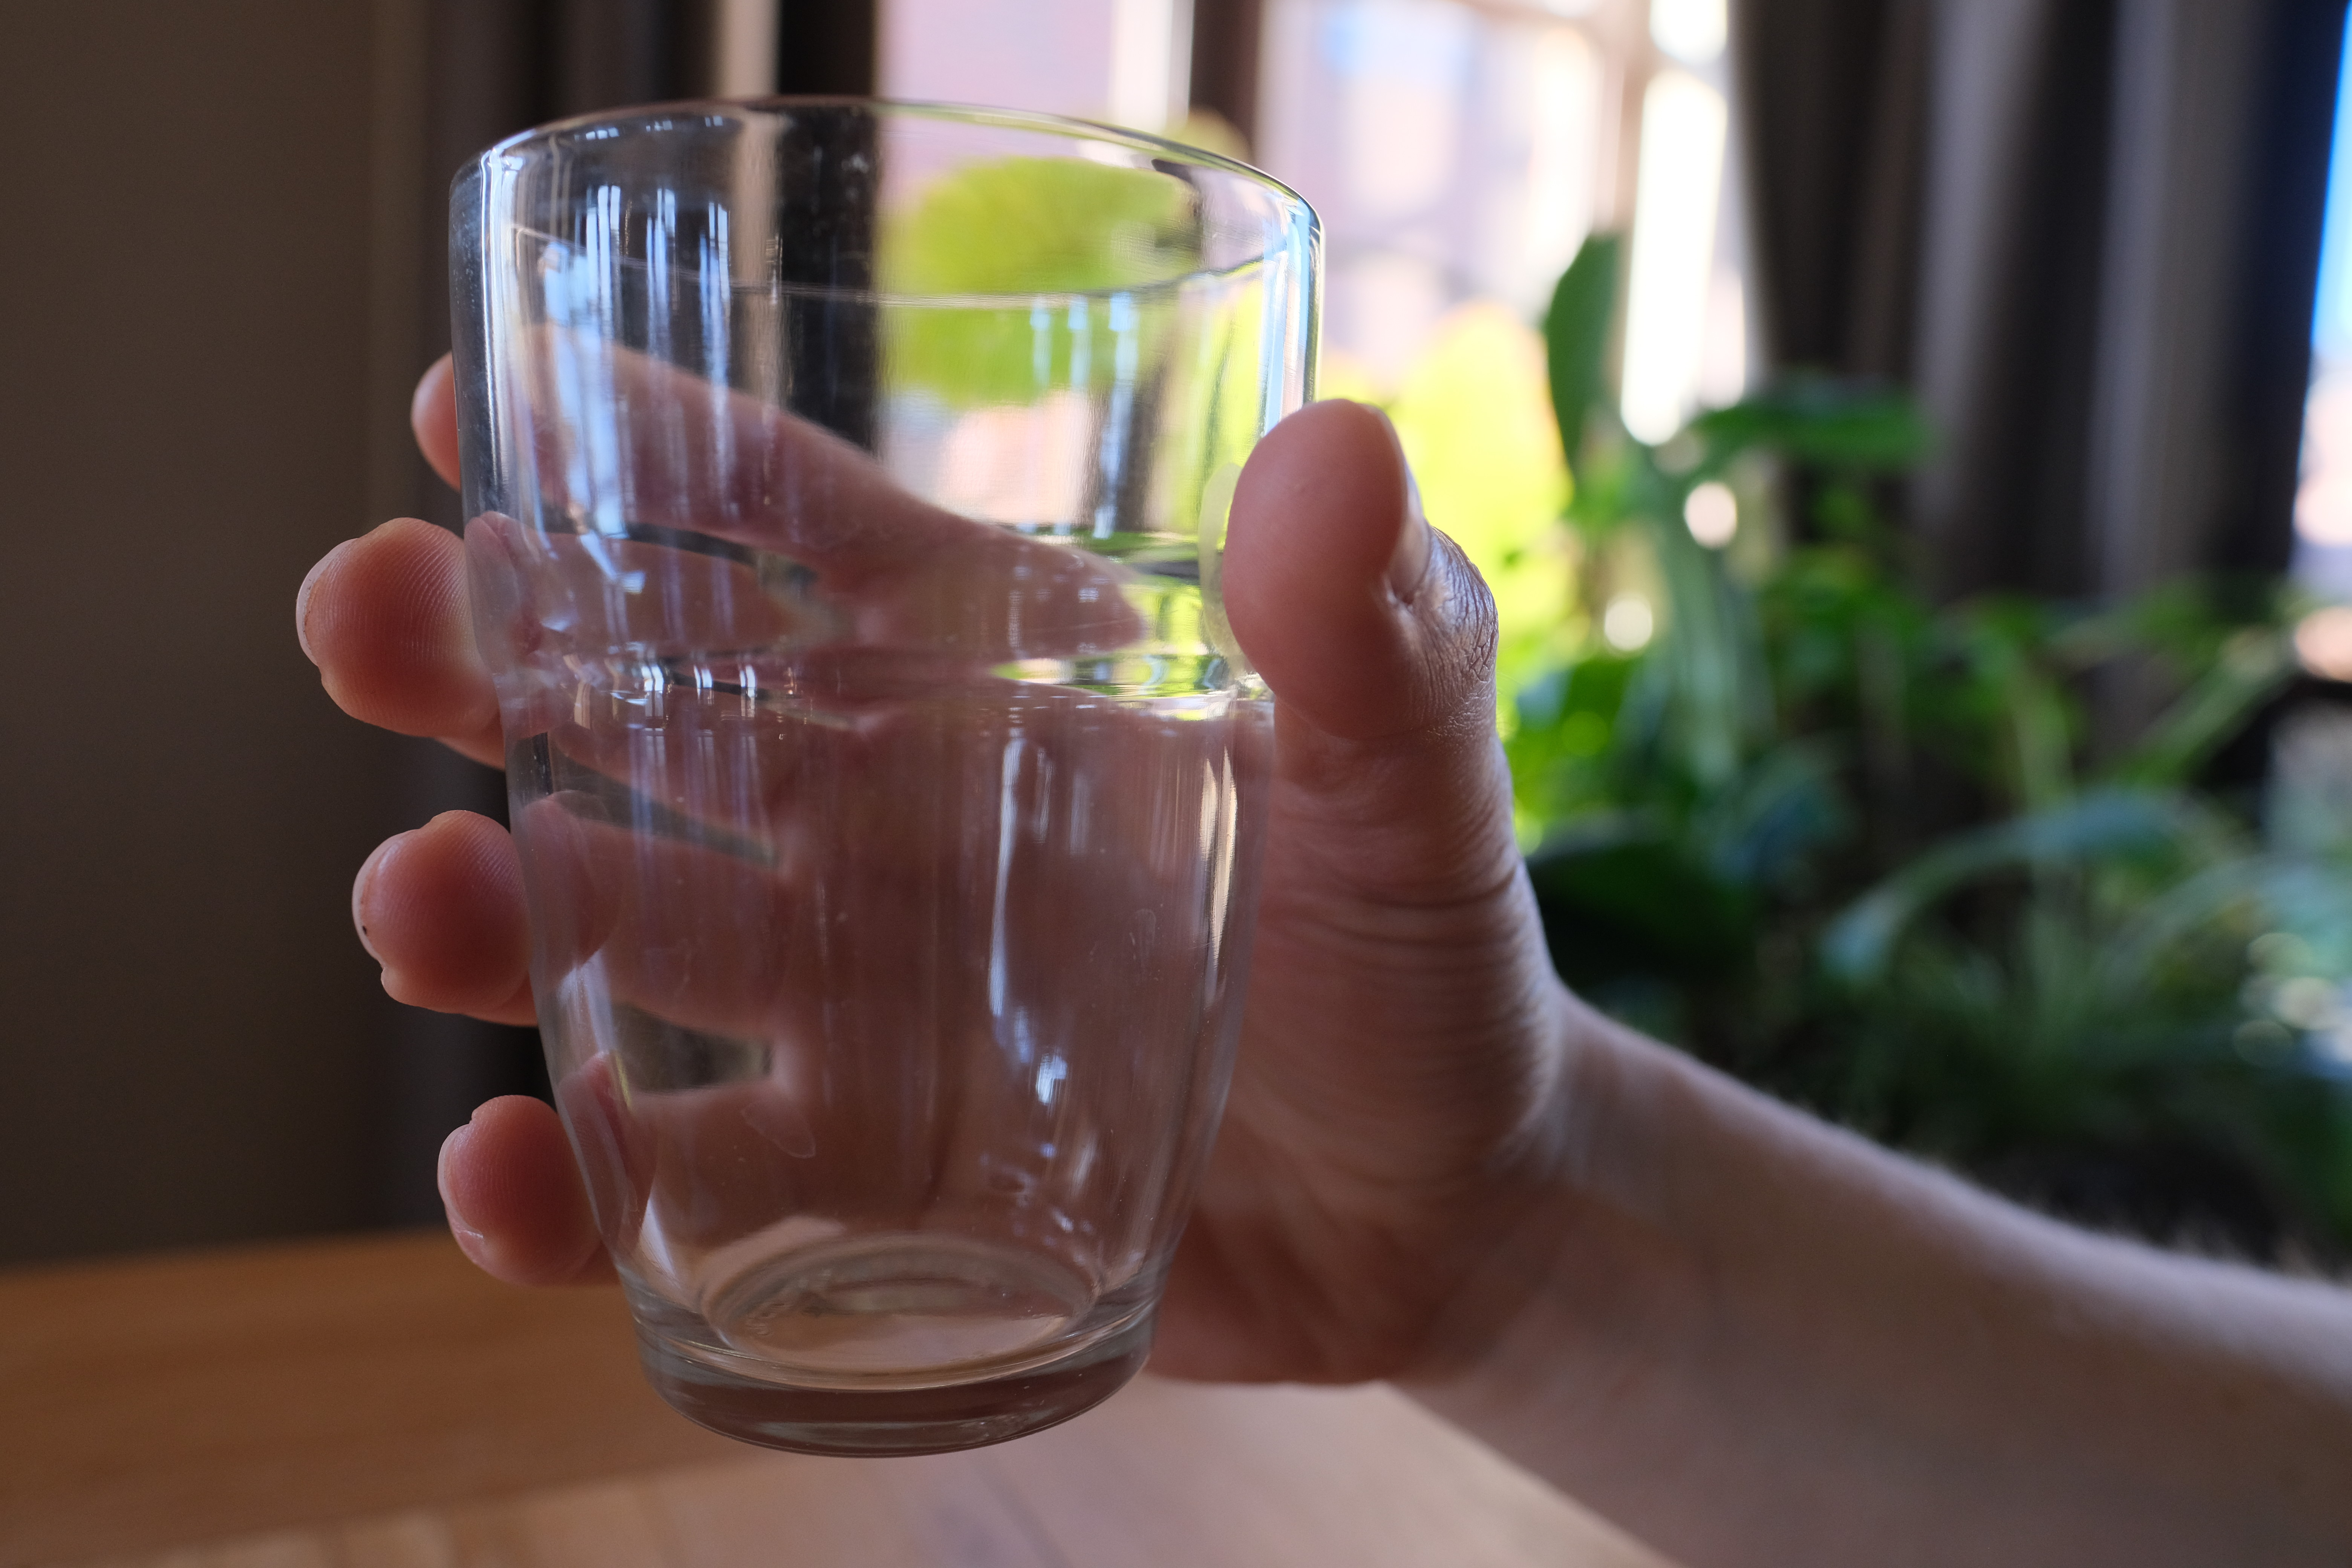
\includegraphics[keepaspectratio, width=\textwidth]{figures/fig_glass.jpg}
        \caption{}
        \label{fig:force_closure_deform_object_glass}
    \end{subfigure}
    \par\medskip
    \begin{subfigure}[b]{0.95\textwidth}
        \centering
        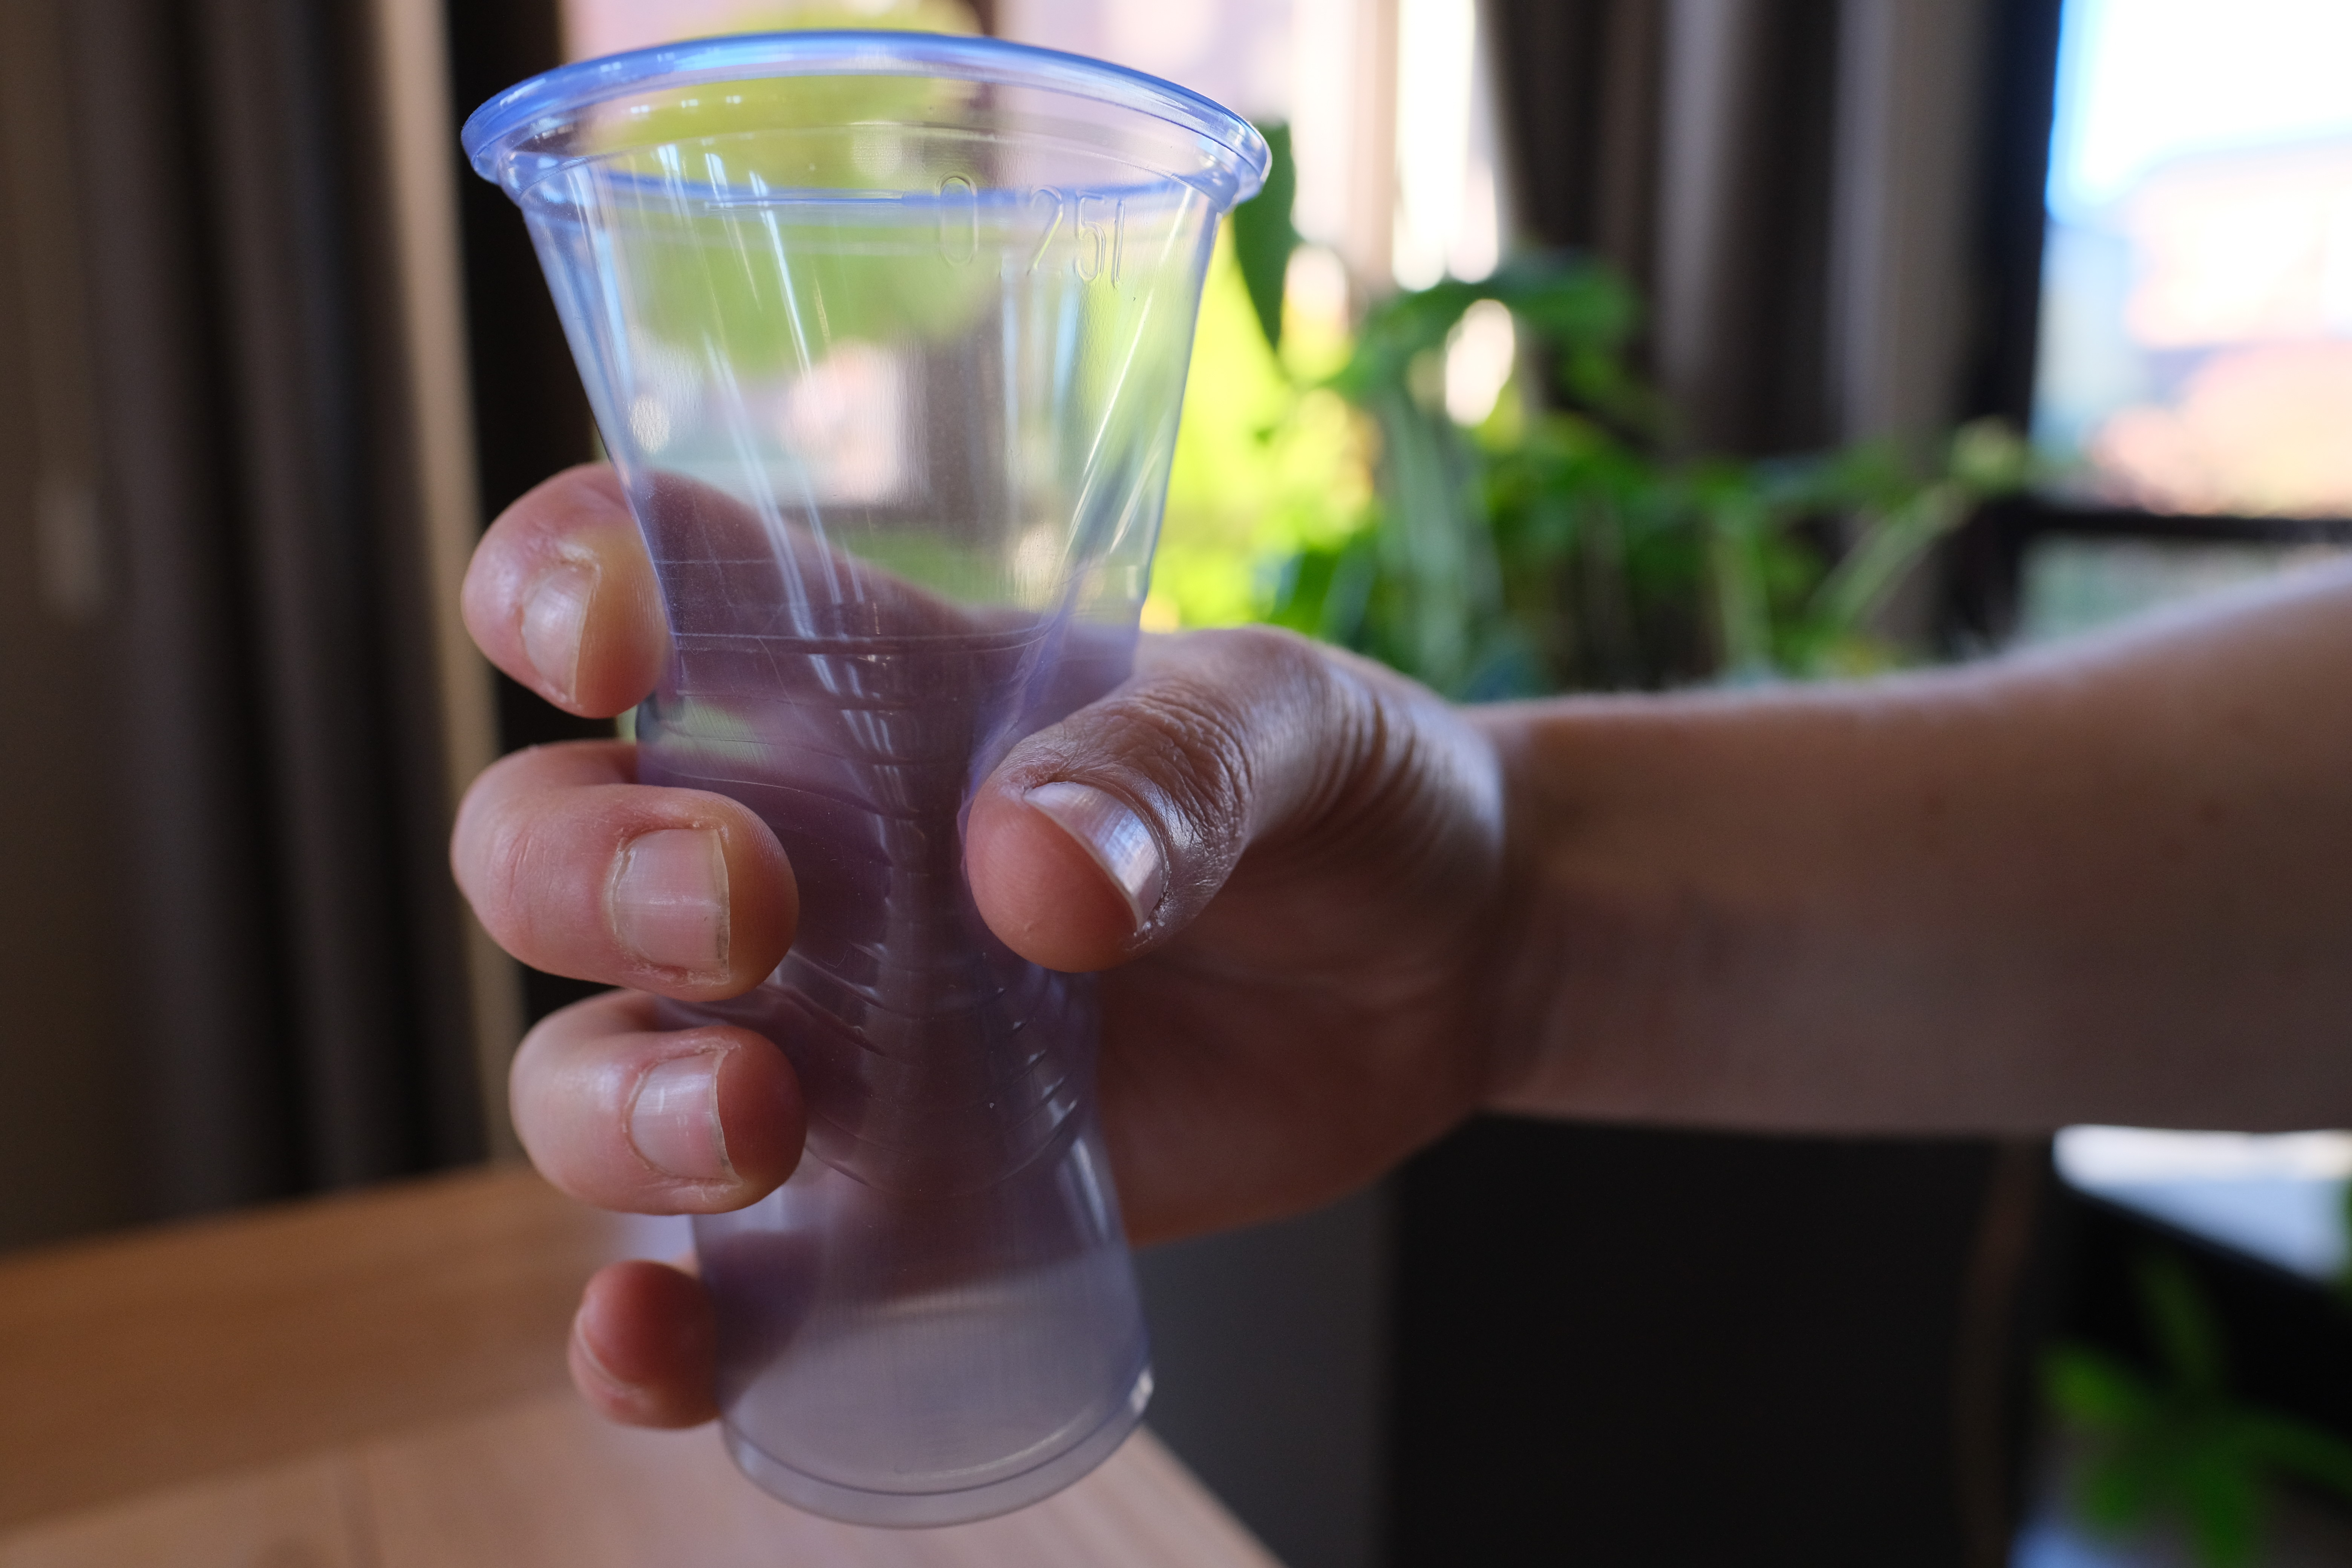
\includegraphics[keepaspectratio, width=\textwidth]{figures/fig_cup.JPG}
        \caption{}
        \label{fig:force_closure_deform_object_cup}
    \end{subfigure}

    \caption[Force closure examples.]{Force closure on a rigid glass (a) and a deformable, plastic cup (b). The deformations of the plastic cup need to be taken into account when calculating a grasping pose.}
    \label{fig:force_closure_deform_object}
\end{figure}

\subsection{Deformable objects: definition, categorization, tasks and solutions}
% Vervormbare objecten: wat zijn ze, categorisatie, welke taken en welke oude pipelines bestaan er
A deformable object is an object whose shape changes when being subject to an external force. This deformation can be temporary and reversible (\textit{elastic}), permanent (\textit{plastic}) or a combination of both (\textit{elasto-plastic}). Deformable objects are found in industrial settings, agriculture and household items. A common categorization \autocite{Saadat2002,Jimenez2012} is based on the geometry of the object: how many dimensions are significantly larger than the other dimensions. The rationale for this categorization is given by small dimensions of the object having a negligible impact on the deformable properties. A canonical example where this property is applied is found in the sheet metal bending industry: the thickness of metal sheets is neglected when computing the required manipulations for bending \autocite{Duflou2005}. A consequence of this categorization is that 3D objects can be considered as 2D deformable objects. For example, both a hollow rubber ball and plush ball can be considered 3D deformable objects based on their dimensionality. However, when considering the dimensions that only impacts the deformable properties, a hollow ball is 2D deformable object as the thickness can be neglected for manipulation. 
\keyWithTitle{Deformable objects}{A deformable object is an object whose shape changes on interaction and can be categorized based on the number of dimensions negligible for manipulation planning.}
In its simplest setting, the deformable object is one dimensional: ropes, strings, cables, threads and catheters, among others. Some of these examples are shown in \cref{fig:dlo_examples}. These objects are also known as deformable linear objects. The term \textit{linear} refers to one dimension being dominant over the other two dimensions. Common tasks for deformable linear objects involve grasping and manipulating ropes, for example, knot tying. Early motor control architectures for solving tasks regarding deformable linear objects used either an open-loop approach or simple visual servoing to execute the motion. An early work clearly demonstrating modular control pipelines is the project of~\citeauthor{Inaba1987} in~\citeyear{Inaba1987}. Their method employs visual servoing for manipulating a rope into a ring and then tying the rope. 
Their perception module uses stereo images to detect the rope and the ring. The planning module is hard-coded to iterate through a set of predefined steps while using the detected centre of the ring and 3D coordinates of the endpoints of the rope from the perception module. An inverse kinematics module provides a target trajectory to the low-level controller. Similar modular pipelines can be found in \autocite{Remde1999} for grasping a rope and in \autocite{Saha2007} where knots are tied with needles using probabilistic trajectories of the rope from a simulated model. Incorporating motion primitives, i.e.\ a predefined set of motor actions corresponding to high-level actions, in the planning module is used in \autocite{Yamakawa2008, Vinh2012} to tie knots in a rope.

\begin{figure}[htbp!]
    \centering
    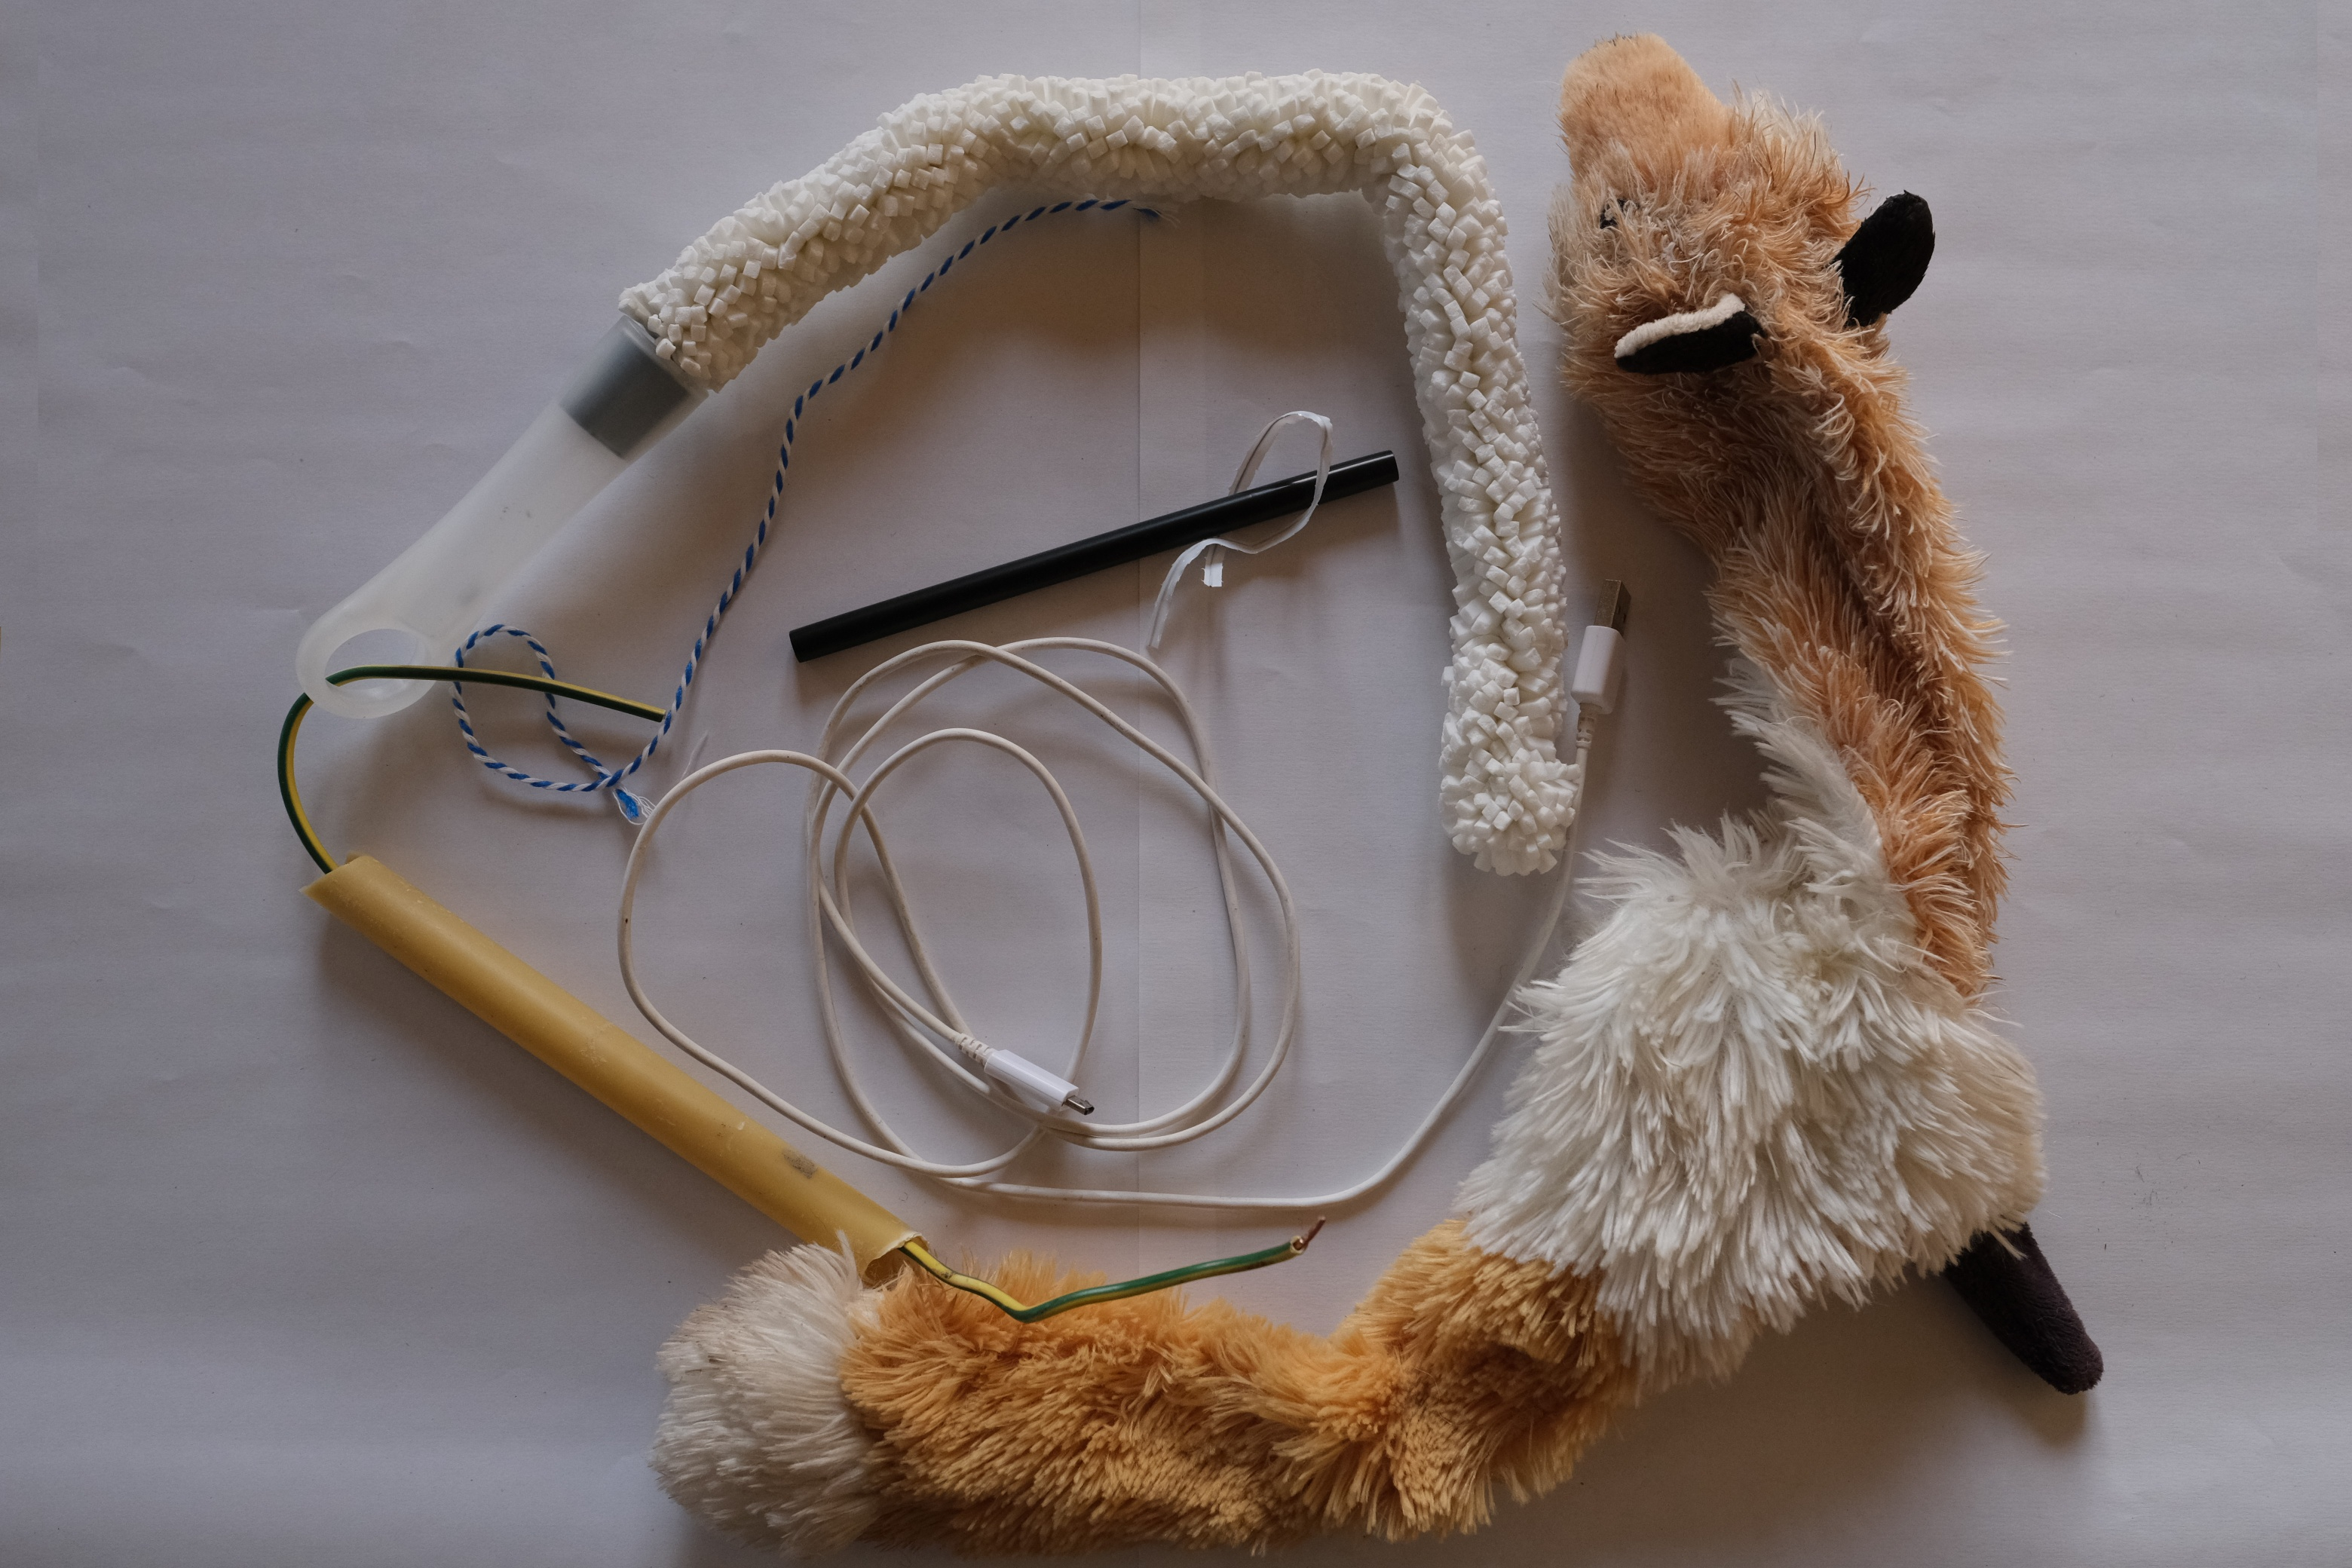
\includegraphics[keepaspectratio,width=\textwidth]{figures/fig_dlos.JPG}
    \caption[Real-life examples of deformable linear objects.]{Examples of deformable linear objects and an application of putting an electrical wire into a rigid pipe.}
    \label{fig:dlo_examples}
\end{figure}

% 2D objects klassieke pipelines
Deformable \textit{linear} objects become deformable \textit{planar} objects when two dimensions are significantly larger than the third dimension. 
In this case, the planning module can disregard the thickness of the material for manipulation. Canonical examples are given in \cref{fig:planar_deform_objects_examples} and contain objects such as clothing, thin-shelled objects like plastic bottles, fabric, paper, and plastic bags, deformable sheets, cards and foam materials. A classic example of paper folding is robotic origami, in which a robot has to sculpt a piece of paper into the desired shape by folding. This problem was tackled with an open-loop control architecture in \autocite{Balkcom2008} to produce a folded hat. \Textcite{Elbrechter2012} takes this a step further by using vision, simulation and fiducial markers on the paper to grasp and fold a paper with a five-fingered end-effector. Related to origami is carton folding and metal sheet bending. Typical control strategies \autocite{Liang1999,Liu2003,Aomura2002} consist of finding the correct locations and sequence of bending operations by modelling the object as a collection of panes articulated through hinge joints. Robotic manipulation of bags has been less studied due to the complexity of modelling and manipulating bags. To circumvent this complexity, dedicated hardware has been researched for grasping \autocite{Kazerooni2005} and unloading \autocite{Kirchheim2008} sacks. A general-purpose two-fingered robotic gripper is used in \autocite{Klingbeil2011} to grasp objects from a table, search the barcode and drop the object into a bag. The planner uses 3D points clouds of depth images taken by a camera. However, they assume the bag is already open for insertion and do not consider any possible deformations caused by touching or dropping an item into the bag.

In the context of this research, it is of interest to note that garments satisfy the same geometrical property of having one negligible dimension as objects such as paper and plastic bottles. However, the main characteristic distinguishing cloth is the compression strength: compared to other two-dimensional deformable objects, cloth does not possess any significant compression strength. Given that the current work deals with manipulations of clothing items, we dedicate \cref{sec:lit_cloth_folding_pipelines} to elaborate on cloth manipulation pipelines.

\begin{figure}[htbp!]
    \centering
    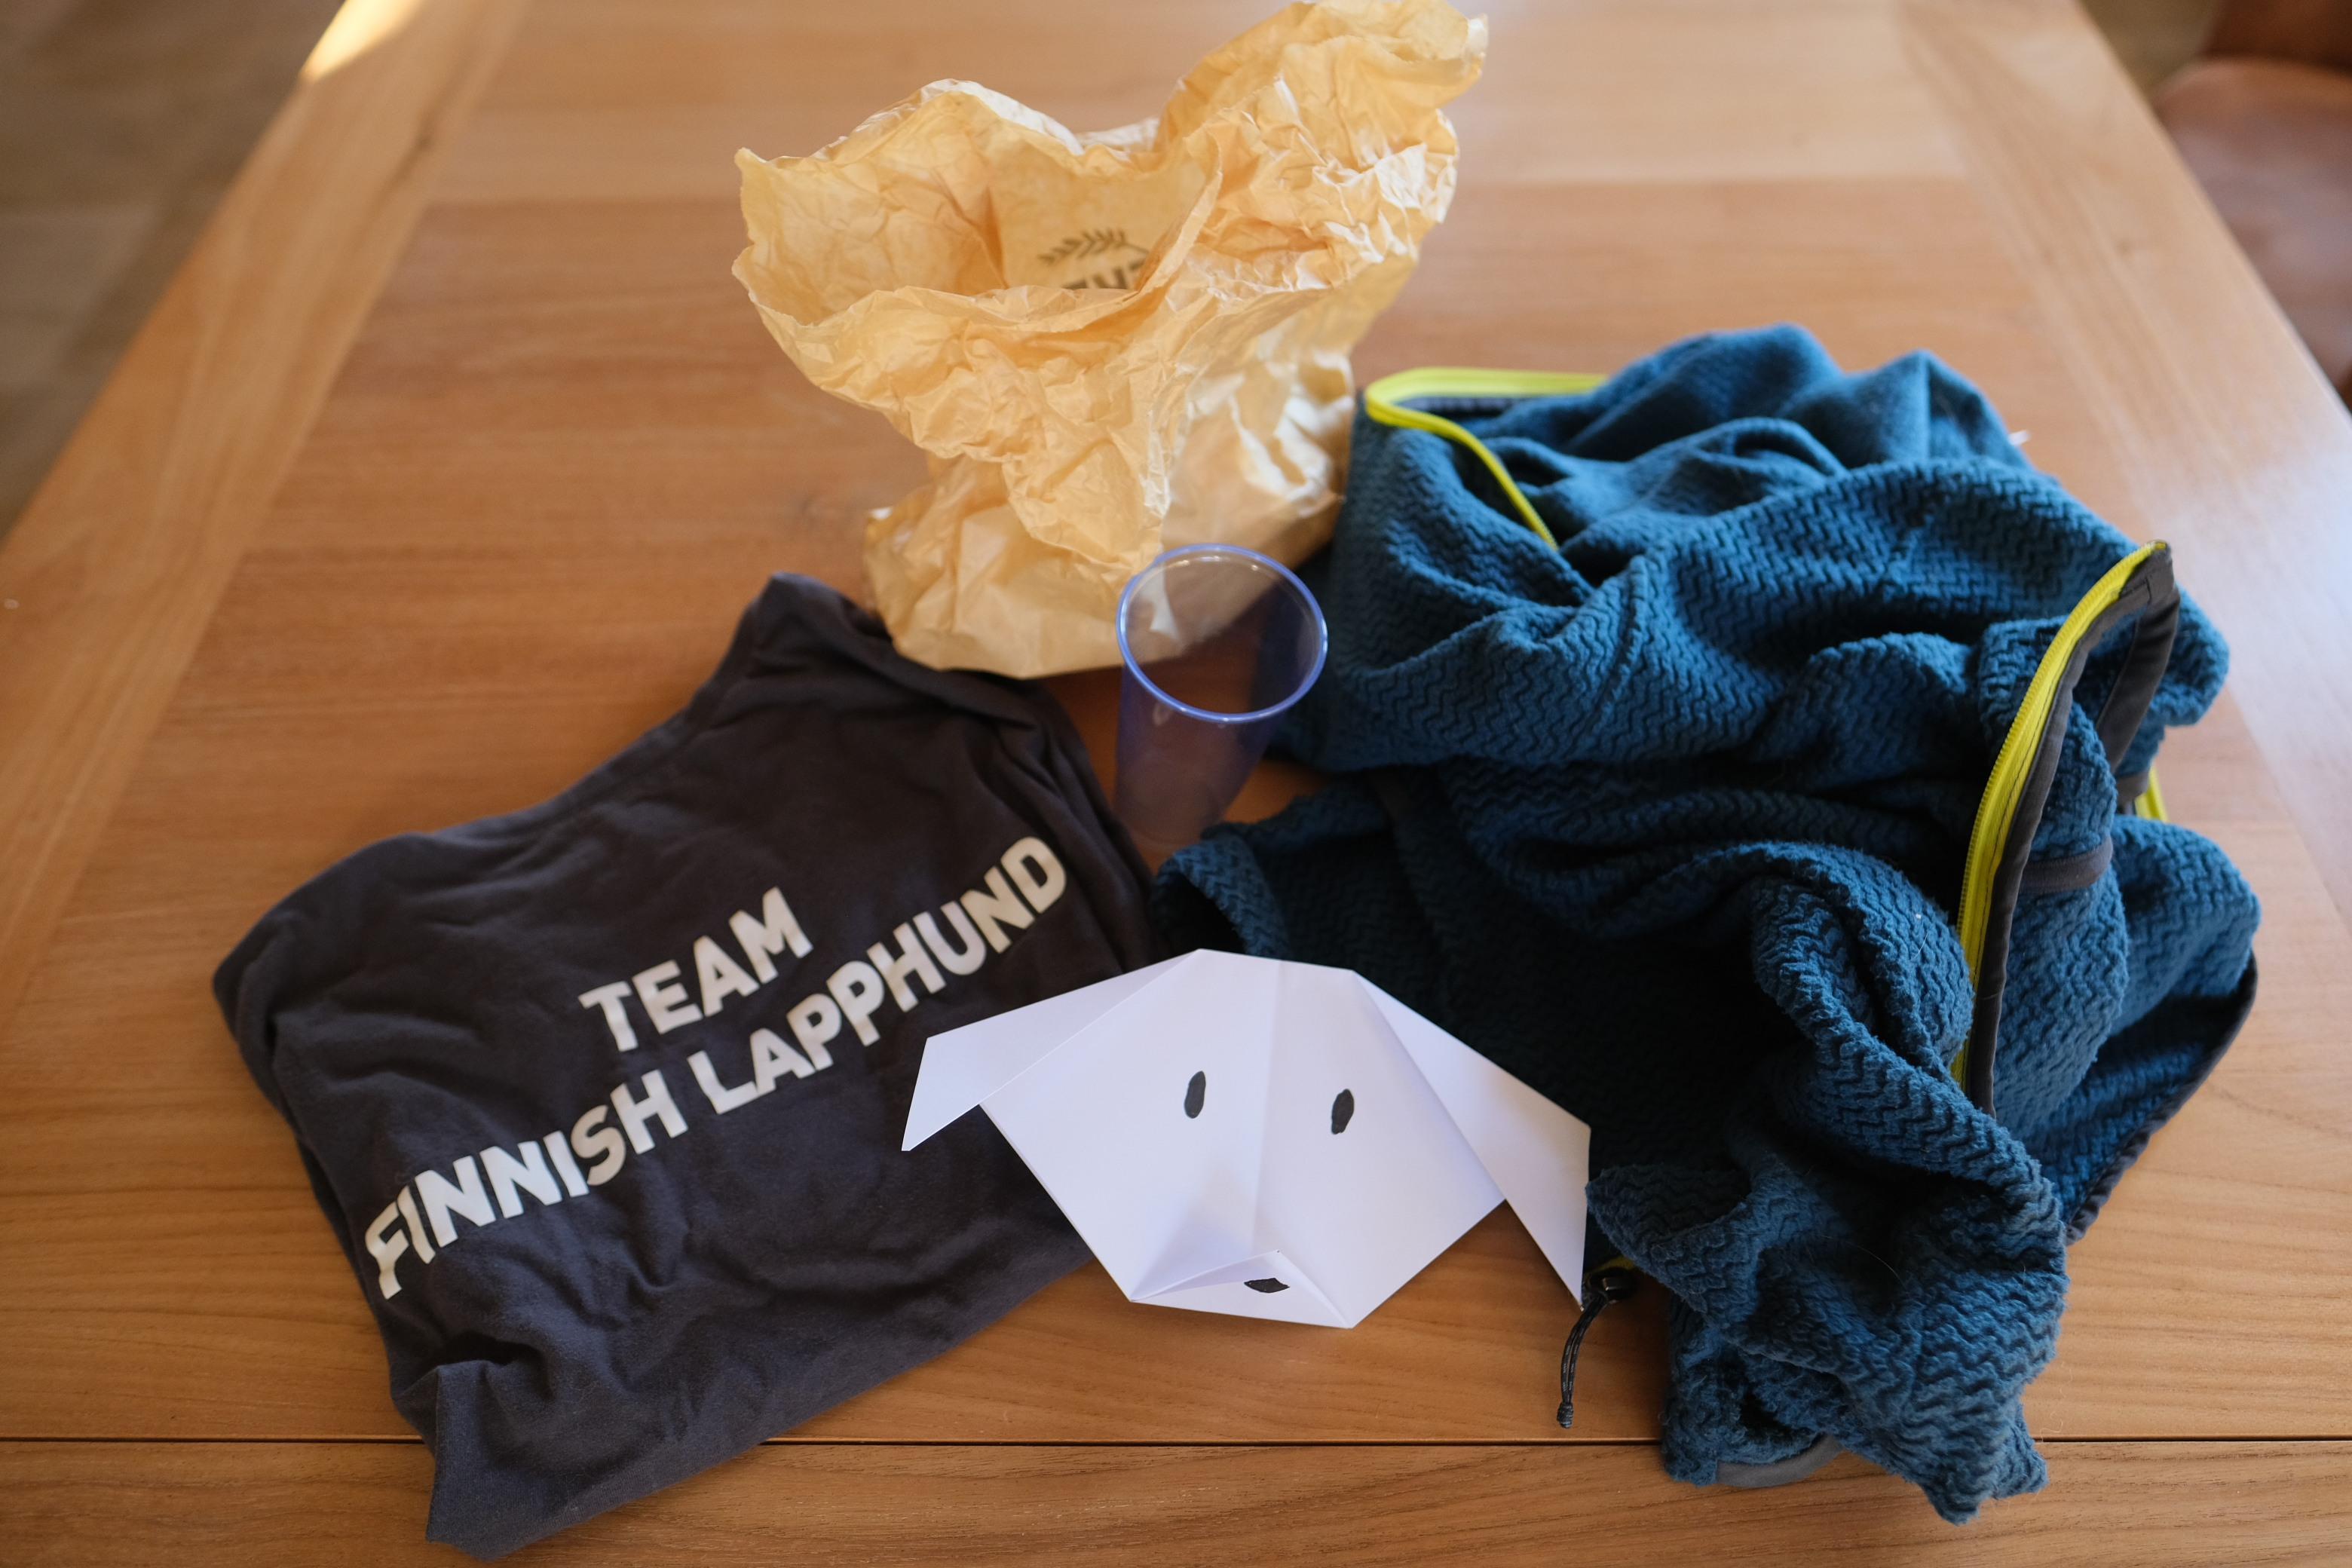
\includegraphics[keepaspectratio,width=\textwidth]{figures/fig_2d_deformables_ex.JPG}
    \caption[Examples of 2D deformable objects]{Examples of 2D deformable objects: origami, paper bag, shirt, jumper and a cup.}
    \label{fig:planar_deform_objects_examples}
\end{figure}

% 3D objects klassieke pipelines
The final category of deformable objects is \textit{volumetric deformable objects} whose deformations across all dimensions of the object are of relevance. Some examples are shown in \cref{fig:volumetric_deform_objects_examples}: objects such as food, plush toys and sponges. In the case of food products, deformations can be caused by both grasping and processing operations such as slicing. In general, 3D deformable objects are the least researched type of deformable objects \autocite{Sanchez2018}. An exception to this is soft tissue, which is important for medical application. We refer the reader to the review paper by \textcite{Taylor2016} for an overview of medical robots in surgery applications. An overview of robotic manipulation of food products is given in \textcite{Chua2003}.

\begin{figure}[htbp!]
    \centering
    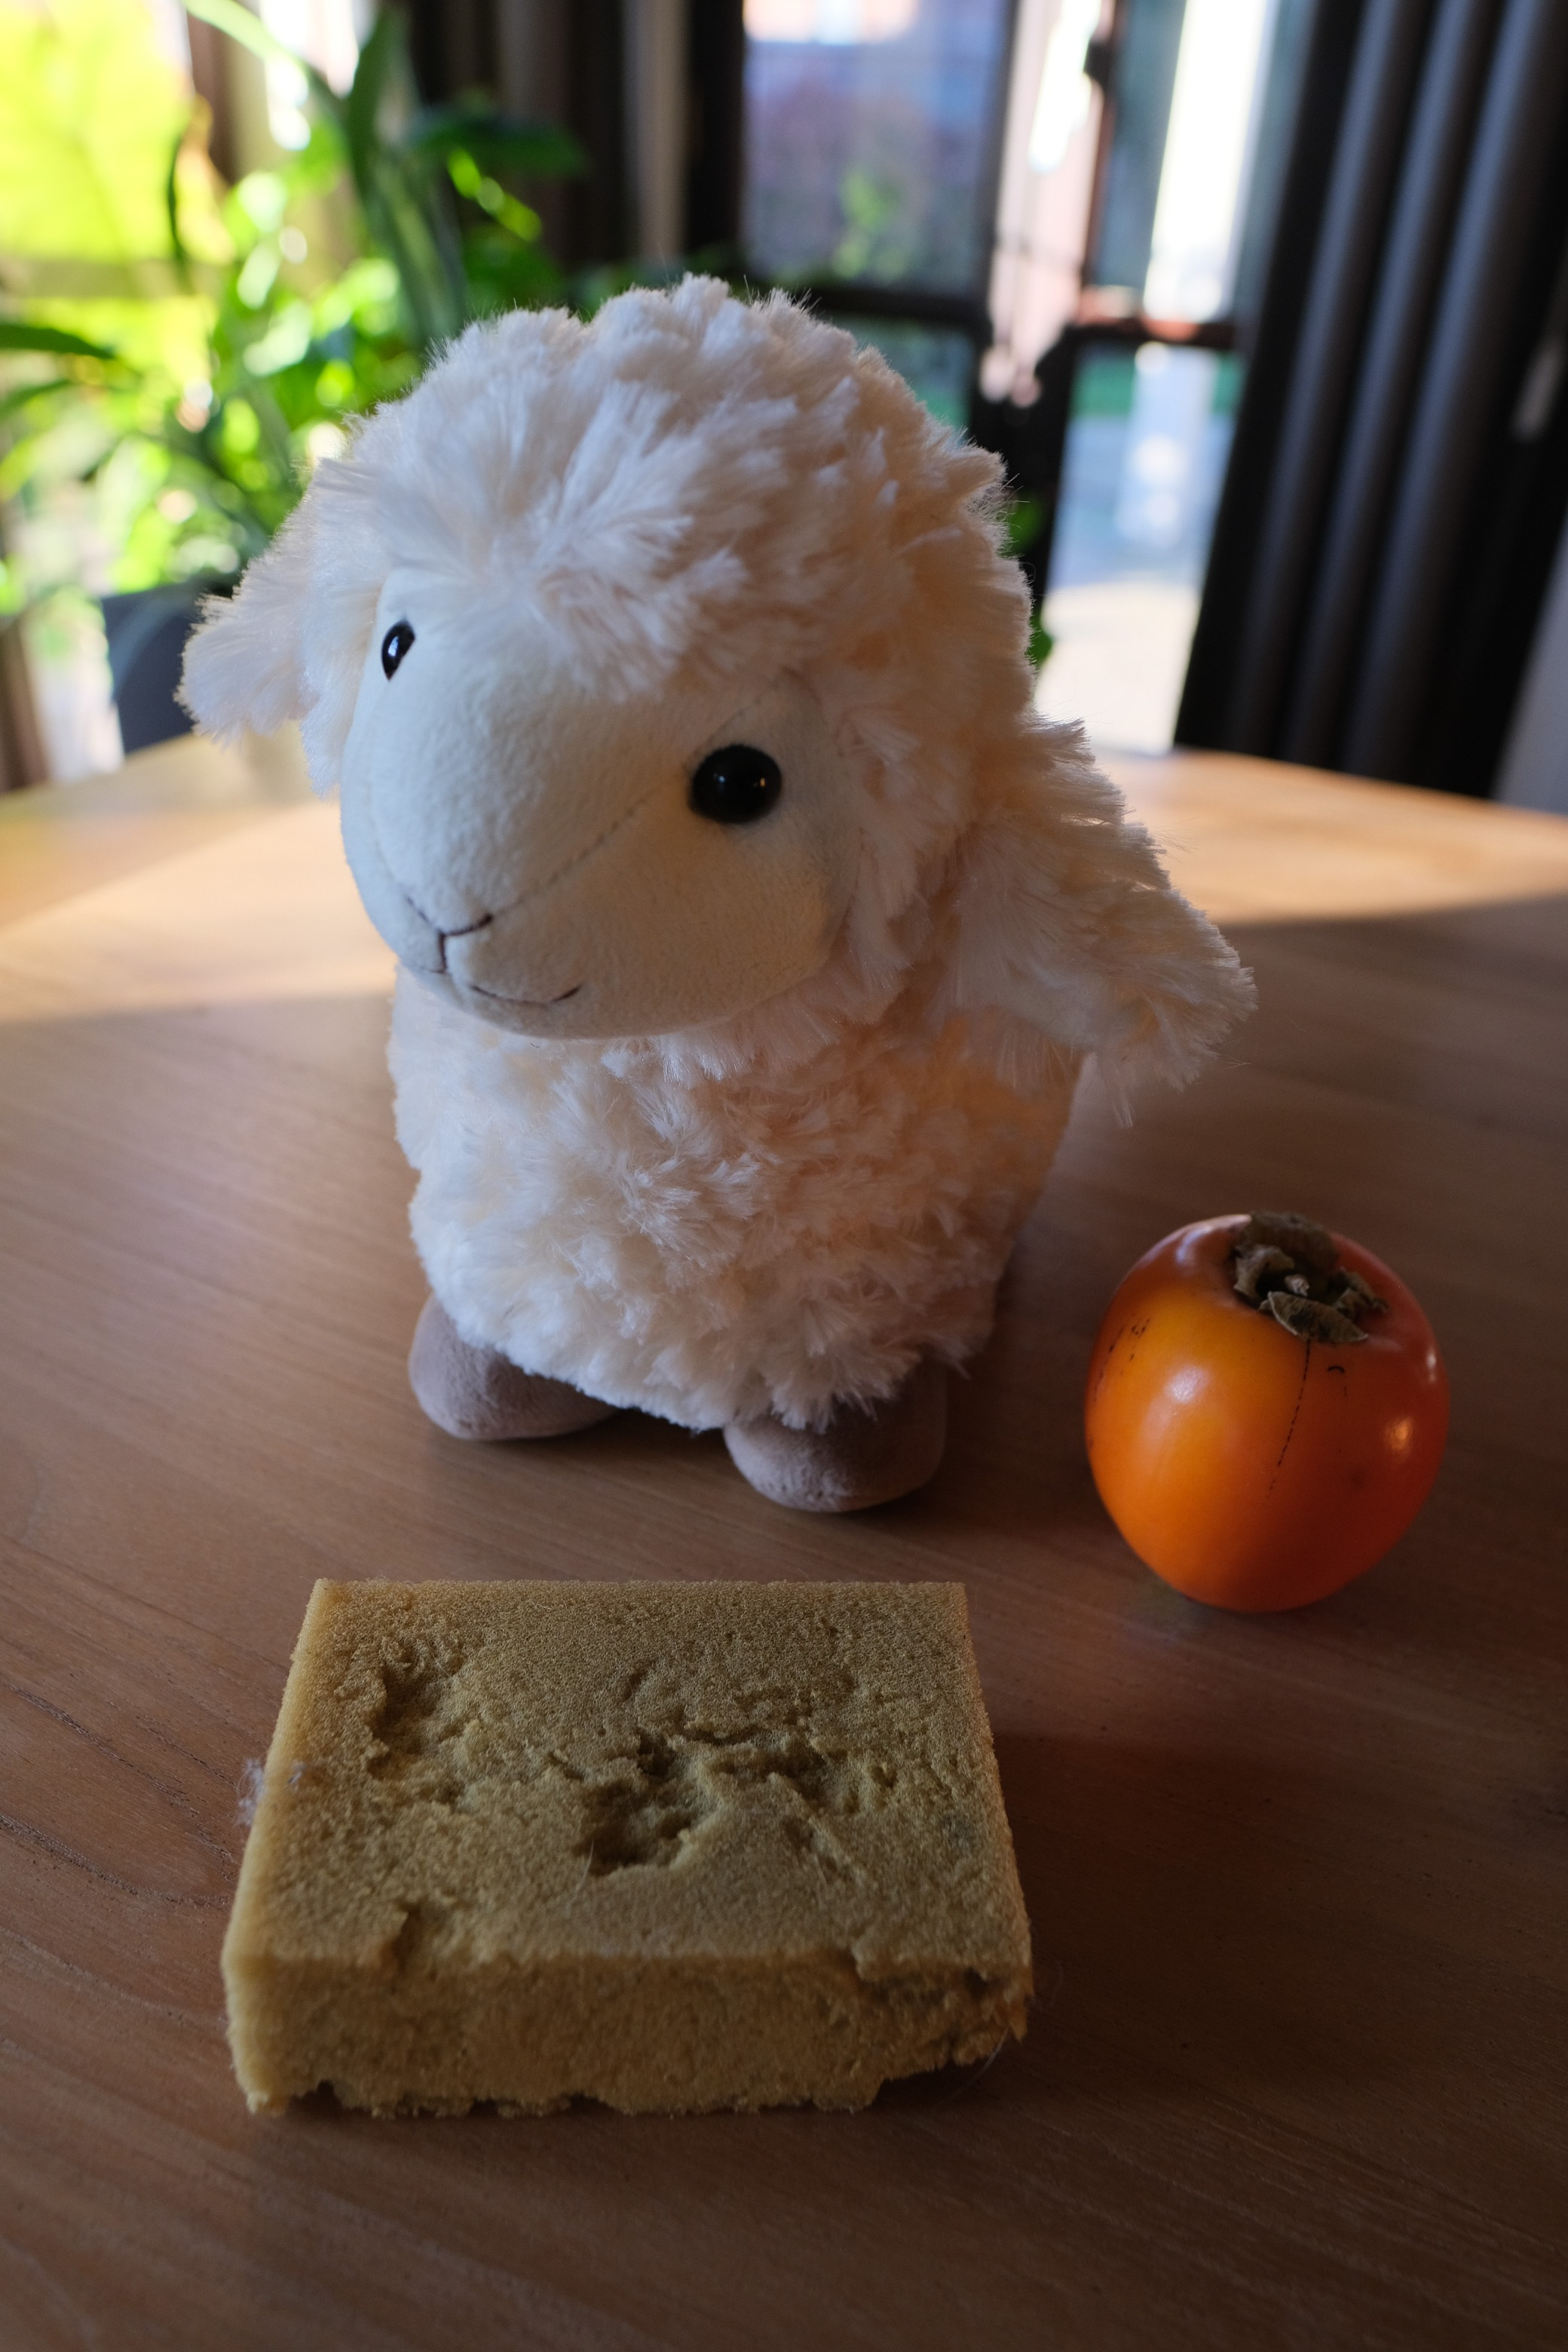
\includegraphics[keepaspectratio,width=\textwidth]{figures/fig_3d_deformables_ex.JPG}
    \caption[Solid deformable objects]{Examples of volumetric deformable objects: sponge, fruit and plush toy}
    \label{fig:volumetric_deform_objects_examples}
\end{figure}

\section{Learning-based approaches to robotic manipulation} \label{sec:lit_learning}

Machine learning, a domain of artificial intelligence, is the study of algorithms that give computers the ability to learn from and make predictions based on data. For robotics, learning provides a way to deal with the inherent systematic as well as random errors in robotic systems and variability in unstructured environments. This is because in learning, you optimize for the grasping task, which implicitly adapts the behaviour to imperfections in the system such as inaccurate sensor readings.

In this section, we provide a short review on the fundamentals of relevant machine learning techniques. We aim to provide background material on \acrfull{DRL}, i.e. the method used in this thesis. To do this, we introduce supervised learning methods (\cref{subsec:lit_sl}), deep neural networks (\cref{subsec:lit_dnn}) and reinforcement learning (\cref{subsec:lit_rl}). We discuss their relevant applications in robotic manipulation with a focus on the manipulation of deformable objects. %For a comprehensive view on the machine learning field, the reader is referred to~\autocite{Hastie2001} and~\autocite{Bishop2006}.

\subsection{Supervised learning} \label{subsec:lit_sl}

% --- SL uitleg ----

\newcommand*{\prob}{\mathrm{P}}

Supervised learning is a machine learning paradigm that operates under the setting where there is a set of \textit{input} variables, for example image pixels, that exert influence over other \textit{output} variables, for example whether there is shirt or trouser in the image.
The components building up a machine learning system are the dataset, the model, loss function and optimization algorithm.
More formally, we can denote the input data as a set $\mathcal{X}$ consisting of vector $x^{(i)} \in \mathcal{X} $ with the superscript $i$ referring to the $i$th observation. In the machine learning domain, this set of predictor variables is called \textit{features}. The set $\mathcal{Y}$ contains the output variables $y^{(i)} \in \mathcal{Y}$. Concatenating tuples of
$\left\{\left(x^{(i)}, y^{(i)}\right) , i \in 1,\dots,N \right\}$
, often called \textit{examples}, leads to a dataset which can be used for learning. Central in this learning procedure is the idea of \textit{function approximation} in which a function $f$, parametrized by $\theta$, maps an input $x^{(i)}$ to its corresponding output $y^{(i)}$:

\begin{equation*}
	f(x;\theta): \mathcal{X} \mapsto \mathcal{Y}.
\end{equation*}

This mapping, also called \textit{model} or \textit{hypothesis}, comes in many forms such as linear models, tree-based methods, support vector machines and neural networks\footnote{We refer to~\textcite{Murphy2012, Bishop2006, Hastie2001} for a thorough exposition on traditional supervised learning methods.}.
The goal of the learning procedure then becomes to adjust the parameters $\theta$ of the model such that a certain performance measure $\mathcal{P}$ is optimized. This metric, called \textit{loss function} $\mathcal{L}$ in machine learning jargon, is specific to the task and domain in which the learning is taking place. In robotic folding for example, the robot might be presented with a candidate grasping pose $\mathbf{u}$. The robot than has to predict the probability $\hat{y} = Q_{\theta}(\mathbf{u}, \mathbf{x}) = \mathbb{E}\left[ \mathcal{S} | \mathbf{u}, \mathbf{x} \right]$ of successfully grasping (success denoted with $S$) a shirt, given some input image $\mathbf{x}$\footnote{This example also implies a heavy assumption; the availability of a dataset containing tuples of (grasping pose, object configuration, probability of success).}.
In this situation, one could minimize the negative cross-entropy loss:
\begin{equation*}
	\mathcal{L}=-y^{(i)} \cdot \log \hat{y}^{(i)} +\left(1-y^{(i)}\right) \cdot \log \left(1-\hat{y}^{(i)}\right),
\end{equation*} with $\hat{y}^{(i)} = f(x;\theta)$ being the predicted output of the model for observation $i$.
The optimization problem then becomes to adjust the parameters $\theta$ of the model $f$ using the examples $\left(x^{(i)}, y^{(i)}\right)$:
\begin{equation*}
	\theta^{*}=\underset{\theta}{\argmin} \: \mathbb{E}_{p(S, \mathbf{u}, \mathbf{x})}\left[\mathcal{L}\left(S, Q_{\theta}(\mathbf{u})\right)\right].
\end{equation*}
The dominant way for heavy parametrized functions such as neural networks to optimize this objective, is to use gradient descent. The gradient expresses the direction of the steepest decrease of the loss function $\mathcal{L}$ with respect to the model parameters $\theta$. By iteratively updating the parameters in the opposite direction of the gradient, in the case of a minimization objective, we gradually arrive at a local or global minimum:
\begin{equation*}
	\theta_{j}:=\theta_{j}-\alpha \frac{\partial}{\partial \theta_{j}} \mathcal{L}(\theta).
\end{equation*}
$\alpha$ determines how large steps we take towards the estimated direction of the closest local minimum. Adaptive methods such as Adam~\autocite{Kingma2014} allows taking variable step sizes per variable based on the historical directions of the gradient.

Supervised learning is an important paradigm for robotic learning because labelled data provides a clear learning signal. This is important because time spent on robots is expensive. Contrarily, the learning signal in reinforcement learning(\cref{subsec:lit_rl}) often does not optimize for direct task performance and might lead to expensive learning times on physical robot platforms. In the following paragraphs, we discuss relevant work in applying machine learning methods for solving robotic manipulation tasks. Generally speaking, there are two main strategies for applying supervised learning in the robotic manipulation pipeline: (1) as perception module or (2) to map states to actions using imitation learning. We postpone the discussion of the application of deep neural networks in robotics after introducing neural networks in~\cref{subsec:lit_dnn}.

\paragraph{Traditional ML methods - Perception}
Traditionally, supervised learning methods are leveraged in the perception module of a robotic manipulation pipeline. For rigid body manipulation, the popularity of data-driven grasp synthesis approach took off with the work of~\textcite{Saxena2008}. There, a logistic regression classifier is trained on synthetic data using manually engineered features. This way, they demonstrate that a robot is able to unload a dishwasher. In the domain of deformable object manipulation, ~\textcite{Ramisa2012} searches for quality grasping points of crumbled cloth in order to maximize the unfolding upon lifting. They do this by first labeling a dataset of shirts with bounding boxes containing the suitable grasping points. Next, they train a logistic regression model to obtain the probability of the desired grasping point in a given bounding box using a bag of features from the input image. By employing the logistic classifier in a sliding window over the image, they give image patches containing local peaks to an \acrshort{SVM} to obtain more accurate grasping candidates. The candidate patch is converted to 3D space by working in a calibrated environment, and motion planning is executed using inverse kinematics. Similarly,~\textcite{Wang2011} folds socks by having a perception system that uses manually engineered features for training an \acrshort{SVM} with Gaussian kernel to determine the type of sock in front of the robot. The deformable nature of cloth leads to self-occlusions making the garment type and pose classification ambiguous. The presence of this hidden state is explicitly modelled using a \acrshort{HMM} in~\autocite{Cusumano2011}. \acrshort{SVM} have also been used for the purpose to identify garment category and pose~\autocite{Li2014, li2014volum}. Learning methods are also being used to find regions of interests on the cloth. For example,~\textcite{Doumanoglou2016} use random forests to learn garment-specific grasping point. In~\autocite{Maitin2010}, RANSAC~\autocite{RANSAC} is used to find the corners of the cloth. These corners are good candidate grasping points for unfolding and identifying the type of cloth. Nearest neighbors have been used to identify wrinkled regions in a washcloth in order to flatten it~\autocite{Willimon2011}.

\paragraph{Traditional ML methods - Imitation learning}
Another strategy to train controllers using supervised learning, is behavioral cloning. Behavioral cloning is a type of imitation learning~\autocite{Argall2009} in which task demonstrations are used for learning task execution. In behavioral cloning, a sequence of states and actions, as executed by a demonstrator, is recorded as dataset for a supervised learning algorithm. The goal then becomes for the model to predict the action a demonstrator would choose, given a certain state. \emph{Voegen we hier nog een degelijkse uitleg toe wat de verschillende LfD aanpakken zijn? Lijkt me relevant om te weten dat methodes zoals kinesthetic-teach-in niet echt nuttig zijn voor cloth domein.} An in-depth view of the field of learning from demonstration is given in~\autocite{Argall2009}. In the case of robotic laundry,~\textcite{Jia2019} learns single robotic laundry tasks from imitation: flattening, folding and twisting. In contrast to the large bulk of robotic controllers trained in \citeyear{Jia2019} using neural networks, they represent the controller using random forests~\autocite{Breiman2001}. The rationale is given by the non-parametric nature of random forests to dynamically change the number of leaf nodes based on the given imitation data and new cloth configurations. Example demonstrations are also used in deformable object manipulation to tie knots. ~\textcite{Schulman2016learning} uses example demonstrations for non-rigid warping~\autocite{Chui2003} based on point-cloud registration of the scene to tie knots with a robotic manipulator. The general idea is to warp the demonstrated trajectory to match the current setting, which may vary in initial conditions and knot geometry. Closely related is the work in~\autocite{Morita2003} where examples and solutions strategies from knot theory is embedded to do motor control. Although imitation learning is a viable alternative for learning to manipulate objects, a general problem plaguing imitation learning methods is generalizing to unseen scenarios. In the case of trajectory execution, errors can accumulate drastically leading to task failures. This is why existing methods apply data augmentation, include teacher advice or use reinforcement learning(~\cref{subsec:lit_rl}).

\subsection{Unsupervised learning}

I am unsure whether to really discuss this.  It fits the general flow but it might also be overkill. On the other hand, it is used extensively in our TCN paper given the UMAP projections. It also helps understanding why the TCN self-supervised method is not unsupervised.

Structure:
\begin{easylist}[itemize]
	& Definition
	& Relevance~:
	&& dimensionality reduction: SIFT, HOW, PCA, T-sne, UMAP
	&& clustering

	& Application in learning (very short): input features for learning algo, visualization of embeddings, separation of cloth, ...
\end{easylist}

% Zie ook literatuur van Jia2019 Cloth Manipulation Using Random-Forest-Based Imitation Learning


\subsection{Neural networks} \label{subsec:lit_dnn}
% Zie ook les van Goodfellow van die reading club

Structure:
\begin{easylist}
	& Motivation: representation matters
	& ANN, MLP basics: neurons, activations, nonlinearities, layers, feedforward, recurrent --> ik zou dit kort houden! Is relevant voor softargmax beter uit te leggen van TCN paper.
	& optimization: backpropagation. Is nuttig om te weten omdat training proces van triplet loss training belangirjk is.
	& Breakthrough 2012: GPU, large datasets, training tricks
	& CNNS. Nuttig voor het onderscheid te weten tussen het perceptie en motor control deel van een netwerk.
	& Increasingly abstract representation through deep layers
	&& motivatie voor perceptie module en motoriek module (cfr levine)
	& Applications in robotics:
	&& perceptual module in pipelines
	&& dexnet, google levine paper
	&& cfr review deep learning in robotics
\end{easylist}

\paragraph{Dit stuk zal de algemene, verplichte ANN uitleg bevatten. }
Comprehensive review on~\acrshortpl{DNN}, see the textbook of~\textcite{Goodfellow2016}.

\paragraph{Early NN in deformable object domain}
The earliest work using supervised learning with neural networks for deformable object manipulation is~\textcite{Howard2000}. In their work, they train a small feedforward neural network that learns the required minimum grasping force for lifting a deformable object. They collect the data by iteratively using more lifting force on objects with certain masses, deformability and damping. A similar approach is proposed in~\autocite{Khalil2007} to fuse tactile and vision data in order to learn physical parameters of the deformable object model. In~\autocite{Foresti2004}, fur tails are grasped from a conveyor belt. To segment the different furs present in the image, they train self-organizing maps~\autocite{Kohonen1982} in which neurons compete to be activated by the input signal. This results in disconnected regions of interest that are joined using skeletonization. Finally, a heuristic is used to determine and grasp the largest fur.

\paragraph{Modern NN in rigid body domain which kicked of the other works}
With the breakthrough in deep learning in~\citeyear{Krizhevsky2012} by~\textcite{Krizhevsky2012}, deep neural networks have found their way into robotic manipulation, starting in the rigid body manipulation domain. A successful approach to training deep neural networks in a supervised setting for robotic manipulation is to use \acrshortpl{CNN} as grasp success predictor.~\textcite{Levine2016} train a \acrshort{CNN} on a large dataset of $800.000$ grasping attempts to learn to predict the grasp success probability of a grasping pose, given an input image. To sample candidate grasping points, they employ CEM~\autocite{CEM}. Dex-Net~\autocite{dexnet2} also trains a \acrshort{CNN} to predict the quality of a grasping candidate. This network is trained using a simulated dataset where objects are put into randomized poses on a plane. They use simulation to evaluate different grasping wrenches using analytic grasp metrics. Their model shows impressive generalizability to the real world, on different models not seen during training. The Dex-Net framework has been extended to work with suction grippers~\autocite{dexnet3}, use dual-armed robots~\autocite{dexnet4} and generate grasping candidates in the network~\autocite{Satish2019}.

\paragraph{Modern NN in deformable object domain}

\subparagraph{NN - Learning dynamics model}
One approach to leveraging the expressiveness of deep neural networks in a supervised setting is to train a dynamics model. This  model, often called world model, is obtained by training on $<\text{state}, \text{action}, \text{next state}>$ tuples. The  problem to solve becomes to use the world model in order to find the optimal sequence of actions that brings to given input state to the desired output state. Or in other words, the robot knows \textit{how} to act while the user can tell the robot \textit{what} it should do. To manipulate a rope into a desired shape, for example an S-shape,~\autocite{Nair2017} let the robot make arbitrary manipulations on the rope while recording the state transitions. This data is then used for training the inverse dynamics model. Planning can then be done using the world model by giving transitionary keyframes that define subgoals to the robot. A similar world model is trained in~\autocite{Ebert2018} where the model learn to predict future pixels given the planned actions. The data collection is done in a self-supervised way in which the robot does motor babbling. The trained world model then enables model predictive control in which they show good performance for folding cloth and towels. Whereas the training data for the world model in~\autocite{Nair2017} is given by self-supervision, in~\autocite{Yang2016} the data is given by teleoperating a humanoid robot with a virtual reality headset. This training data is then passed into an autoencoder which produces a time series in latent space. A second stage neural network then learns cloth dynamics by sliding a window over the encoded time series. A further attempt to embed the world model into the control module can be done by sandwiching a fully-connected network between the encoder and decoder~\autocite{Tanaka2018}. Instead of embedding a controller module, other work embed physics priors in to the network architecture. By assuming the deformable objects are build up of small, connected particles, it is possible to represent their connectivity and interactions in a graph neural network. This allows to efficiently learn deformable object dynamics to solve for downstream control tasks such as poking deformable objects~\autocite{Mrowca2018} and merging liquids~\autocite{Li2018}.

\subparagraph{NN - Imitation learning.}
Another way neural networks have been employed for learning robotic manipulation tasks is by giving task demonstrations~\autocite{Ravichandar2020}. Given the cost associated with real robot rollouts, it is beneficial to lower the dataset requirements by having access to the motor control outputs or to decrease the input dimensionality by for example avoiding to learn from pixels. This explains the popularity for teleoperated~\autocite{Zhang2018,Duan2017} and kinesthetic teaching~\autocite{finn2017one} approaches. However, it is difficult to teleoperate a robot or physically manipulate a robotic arm to fold clothing items. This is because the speed and forces associated while executing the task is relevant for achieving proper folds. One method to compensate for this difficulty is to solve the imitation learning task in simulation and trying to transfer it to the real world. This is explored in~\autocite{Seita2020} that generates example demonstrations in simulation and uses behavioral cloning to train a motor policy network to flatten a towel. To fine-tune this policy outside the seen dataset distribution, they employ dataset aggregation (often labeled as DAgger) in which an oracle policy is used to label the unseen states during training. An alternative is given in ~\autocite{Sundaresan2020} that uses simulated data to learn visual object descriptors indicating the segments of a rope. Such embeddings implicitly encodes geometric structure which can then be used for knot-tying using example demonstrations.

% Overgang: rational voor RL
\paragraph{SL - conclusion.}
Framing robotic manipulation of rigid and deformable objects as a supervised learning problem has been successful for estimating the state of deformable objects or manipulating cloth by means of behavioral cloning. However, training with hand-labelled or generated data has two main issues~\autocite{pinto2016supersizing}. The first issue is the human bias towards preferring grasps poses that are similar to the way a person would grasp an object. This discourages exploration of unconventional grasp configurations. The second issue is the cost to exhaustively evaluate all possible grasps because an object can be grasped in multiple ways. Therefore, learning on robots requires a method that can work without human supervision.

\subsection{Reinforcement learning} \label{subsec:lit_rl}

% 		RL BESCHRIJVING: dat kan later adhv RL in robotics: a survey, sutton-barto en A survey of deep network solutiosn for learning control in robotics: from RL to imitation 

% Overview inspiraties:
% 	A survey of deep network solutiosn for learning control in robotics: from RL to imitation
% 	Thesis Jannick , Thomas , Matas? 
% 	
Structure:
\begin{easylist}

	& A Concise introduction to RL
	&& MDP formalisatie
	&&& state action transition reward discount factor
	&&&& model-based vs model-free RL
	&& episodic MDP
	&& State vs observation + markov property
	&& Goal: maximize expected reward
	&& RL loop and elements: state representation, reward function.
	&& Defintion policy
	&& Definition value function, q function
	&& from bellman equation to q-learning
	& contrast to SL: RL is much harder because (1) delayed rewards (credit assign problem) (2) non-stat data, (3)
	%(also check & suttonbarto and thesis NG https://web.archive.org/web/20141222084445/http://www.cs.ubc.ca/~nando/550-2006/handouts/andrew-ng.pdf)
	& why relevant for robotics - RL in the context of optimal control % zie ook RL in robotics: a survey sectie 1.2 p5 EN review of robot learning for manipulation p24 sectie 6.3
	&& model-free: tradeoffs % zie review of robot learning for manipulation met Peter p25
	&& model-based: tradeoffs
	&& Figuur toevoegen. Zie ~\cref{fig:DRL-robotics}
	& RL Flavours
	&& value based methods: q-learning
	&& policy based methods: vermelden maar niet al te diep op ingaan
	&& actor critic methods: vermelden maar niet al te diep op ingaan
	& Where is the DEEP in DRL
	&& DQN
	&&& target network
	&&& experience replay
	&& policy-based and actor critics: DDPG en SAC vermelden
	& Literatuur: Applications in robotic manipulation and cloth

\end{easylist}
\begin{figure}
    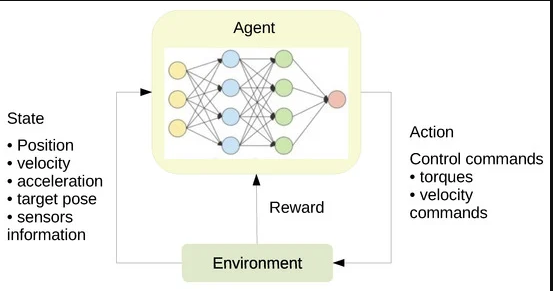
\includegraphics[width=\linewidth]{\home/chapters/02-sota/figures/DRL-in-robotics.png}
    \caption{}
    \label{fig:DRL-robotics}
\end{figure}

Reinforcement Learning is an eminent approach for learning control policies with minimum user intervention. A complete review of RL is outside the scope of this thesis. Therefore, we refer the reader to the standard textbook of~\textcite{Sutton2018}.


% YOU ARE HERE!!!
% Herlees alles hieronder en hang alles nog is deftig aan elkaar.
% Kijk nog is of je structuur niet zou wijzigen en SL - NN stukken zou mergen
% Self-supervised stuk aanvangen. Neem er eerst de 2 surveys bij dat je gevonden hebt. Beschrijf adhv daarvan kort SSL, contrastive learning, copy paste wat uit je TCN paper literatuur en verwerk de papers dat je nog hebt staan. 
% zie ook https://github.com/jason718/awesome-self-supervised-learning
 
\paragraph{Literature.}
Much of the work for learning manipulation skills for deformable objects has been build up work done in the rigid objects domain. These methods in turn often rely on work done on simulated and games environments. First attempts at transferring DQN to visual servoing were attempted in~\autocite{Zhang2015} but failed. Their end-to-end approach to frame the inherent continuous action spaces of robotic manipulation to a discrete algorithm such as DQN is to discretize the joint motor outputs into $9$ motor actions bins. To further reduce the search space, they reduce the amount of joints of the robot from $7$ DOF to $4$ DOF. They train a DQN controller in simulation while adding noise and task variations. However, transfer to real robot failed due to missing simulator realism and appropriate reward functions. Later work~\autocite{James2016} managed to transfer virtually trained DQN agents on pixels by using high-fidelity simulation and careful reward tuning. With the introduction of continuous action spaces for value-based agents, more specifically DDPG~\autocite{Lillicrap2015}, DQN variants started being successfully applied in the robotic manipulation domain~\autocite{Gu2017}. This success was mainly driven by directly representing the continuous action space of robot actuators, reusing past experiences for training and working in parallel.

Deep reinforcement learning for deformable object manipulation has arguably first been used in~\autocite{Matas2016}. By training a DDPG agent in simulation, they demonstrate limited transferability to the real world using domain randomization to fold a towel. They find that a lack of simulation tools for cloth is the main factor limiting their results. ~\autocite{Jangir2020} speed up this approach by warm-starting the learning with example demonstrations but does not transfer to the real world. An additional speed-up can be obtained by filling the replay buffer with example demonstrations~\autocite{Tsurumine2019}. ~\autocite{Wu2020}
examines how to link two policies, i.e. picking and placing cloth which are normally independently trained. They opt for structurally encoding the relationship between picking and placing of cloth. This done by having the second learned policy, i.e. the place policy, receive the last output of the picking policy. This way, the network can optimize the picking point that gives the most value during placing. 


~\autocite{lee2020learning} 
autonomously generates data of a robot manipulating cloth using a motor control heuristic. Such heuristic allows collecting more useful data compared to motor babbling. This dataset is then used in an offline RL setting, also known as batch RL. In contrast to other DQN methods, their network is fully convolutional resulting in a Q value heatmap per possible action. This approach is successful in achieving simple folds in rectangular cloth, without one hour of real world data. 


- ~\autocite{seita2021learning} 
Use Transporter networks, an architecture that predicts the spatial displacement of a local area, to learn to fill bags with objects in simulation. 



\subsection{Self-supervised learning}
cfr TCN paper.

"Nair" approach: learn latent space and solve the task in latent space -> nearest neighbor retrieval in latent space.

Papers:
- Mengyuan Yan et al. Self-Supervised Learning of State Estimation for Manipulating Deformable Linear Objects". In: IEEE Robotics and Automation Letters (RA-L). 2020.
	Uses two autoencoders as dynamics model. One rough and detailed encoder.
	First one:
	use spatial transformers
	coarse-to-fine: iteratively refine estimation of image space coordinates of points on the rope.
	Second one: novel self-supervised learning objective.
	to have better sim2real transfer
	Encode color-contrast cue: assumption of the rope having a different color from the background as a Gaussian Mixture Model.
	You have XY coordinates of points of rope given by first model. You use this to render the rope.  (differentiable renderer). You want this to look very much like the real image you have in front of you. --> train a GMM on this image for background and foreground pixels.
	The second image is color-based segmentation on the real image.
	To make these two image look alike, you define a loss using the GMM produced segmentation and backpropagate it back to the first network.



- Wilson Yan et al. Learning Predictive Representations for Deformable Objects Using Contrastive Estimation". In: Conference on Robot Learning (CoRL). 2020.
	Contrastive objective to learn latent space describing state of a rope. This encoding is used as a forward dynamics model in which an action trajectory is sampled that minimizes the distance towards the given goal state. The actions are chosen such that only points on the rope are considered.

- Visuospatial foresight for multi-step, multi-task fabric manipulation Hoque
	Is ong hetzelfde als hierboven Yan2020
	learned an image prediction model in simulation, which can be used to solve arbitrary goals at test time via Model Predictive Control. They apply domain randomization to transfer fabric smoothing policies to a real-world surgical robot. However, their approach fails to transfer folding tasks successfully due to the sim-to-real gap.

\section{Datasets for robotic learning} \label{sec:lit_datasets}
Motivatie:
	Link met SL
	Link met RL, offline RL

	Kan simulatie of echte data zijn.

Relevante werken:
	a large scale dataset for robotic grasp detection depierre
	cornell grasping dataset
	Kleeberger K, Landgraf C, Huber MF. Large-scale 6D object pose estimation dataset for industrial bin-picking
	DexNet, Levine2016
	CLOTH:
	benchmark paper voor deform object manip Seita

Cloth datasets:
	mnist fashion



~\textcite{Levine2016} generate a dataset of $800.000$ real executed grasps. They record ...
Dex-Net~\autocite{dexnet2} contains an simulated dataset of $6.7$ million robust grasps. They generate a depth image with candidate grasping pose and grasping outcome of $1.500$ meshes.

\section{Simulation environments to accelerate learning} \label{sec:lit_simulation}

Motivatie voor simulatie: dure, trage robot tijd
Componenten: physics engine, robot simulatie, link naar fysische platform.

\subsection{Cloth simulation methods} \label{subsec:lit_cloth_sim}
%Zie ook "Robotic manipulation and sensing of deformable objects in domestic and industrial applications: a survey" p4 voor overzicht om te introduceren maar focus op particle based methods.
%  zie ook Dexterous Robotic Manipulation of Deformable Objects with Multi-Sensory Feedback - a Review van khalil
%  Voor de specifieke methode, zie ook p47 van Seita zijn boek 
\begin{easylist}
	& Wat maakt cloth simulatie moeilijk.
	& Aanpakken tot cloth simulatie (kort de categorisatie)
	&& FEM
	&& particle based
	% & Particle-based simulation
	% && formalisatie 
	% && Integrators
	% && position based dynamics 
	& Ander werk dat gebruik maakt van cloth simulatie voor robotic maniulation.
\end{easylist}


\subsection{Transferring simulation results to the real world}  \label{sec:lit_sim2real}
Structure:
\begin{easylist}
	& sim2real problem uitleggen.
	& Verschillende aanpakken uitleggen:
	&& Meta learning
	&& simulatoin randomization
	&& system identifitcation
	&& domain adaptation
	&& progressive networks (Rusu et al)
	&& James et al: real to sim
	& literatuur bespreken.

\end{easylist}

PAPERS:
System idemtification
In~\autocite{Howard2000}, a mass-spring-damper simulation of deformable object is tuned to the real world by probing the object with the gripper containing a force sensor.


Domain randomization:
Matas2016 for transfering cloth manipulation tasks and Yan2019 for bringing policies to learned in simulation to the real world among others.
\section{Reward learning}  \label{sec:lit_reward_learning}
\begin{easylist}
	& General introduction
	& Motivatie: Reward hacking, impossible to capture all ingredients
	& Literatuur:
	&& 	IRL
	&& 	Reward learning
\end{easylist}

\section{State perception through instrumentation} \label{sec:lit_instrumentation}
Motivatie.
Definitie.
literatuur:


\end{document}